% Every result number comes from assets/ (generated by make_assets.py from results/, data/ and models/); none is typed here.
\documentclass[aspectratio=169,10pt]{beamer}

% ---------- fonts (delete the next two lines to get the default Computer Modern sans) ----------
\usepackage[sfdefault, lining, tabular]{FiraSans}
\usepackage{FiraMono}

% ---------- math, tables, graphics ----------
\usepackage{amsmath, amssymb}
\usepackage{booktabs}
\usepackage{tabularx}
\usepackage{graphicx}
\usepackage{tikz}
\usetikzlibrary{arrows.meta, positioning, shapes.geometric, calc}
\usepackage{appendixnumberbeamer}
\usepackage[authoryear, round]{natbib}
\graphicspath{{assets/}{assets/screenshots/}}

% ---------- colors: the palette of the Streamlit demo ----------
\definecolor{accent}{HTML}{003299}      % ECB blue
\definecolor{amber}{HTML}{B26A00}
\definecolor{softgrey}{RGB}{100, 100, 100}
\definecolor{dovish}{HTML}{2F5DA8}
\definecolor{hawkish}{HTML}{B26A00}
\definecolor{neutral}{HTML}{6B7280}
\definecolor{irrelevant}{HTML}{A3A8B3}

\setbeamercolor{structure}{fg=accent}
\setbeamercolor{title}{fg=accent}
\setbeamercolor{frametitle}{fg=accent}
\setbeamercolor{block title}{fg=white, bg=accent}
\setbeamercolor{block body}{bg=accent!5}
\setbeamercolor{itemize item}{fg=accent}
\setbeamercolor{itemize subitem}{fg=accent}
\setbeamercolor{enumerate item}{fg=accent}
\setbeamercolor{alerted text}{fg=amber}
\setbeamercolor{section in head/foot}{fg=accent}
\setbeamercolor{footline}{fg=gray}
\setbeamercolor{footnote}{fg=softgrey}
\setbeamercolor{bibliography entry author}{fg=accent}
\setbeamercolor{bibliography entry note}{fg=softgrey}

\setbeamertemplate{frametitle}[default][left]
\setbeamerfont{frametitle}{series=\bfseries, size=\large}
\setbeamerfont{section in head/foot}{size=\scriptsize}
\setbeamerfont{footline}{size=\scriptsize}
\setbeamertemplate{itemize item}{$\bullet$}
\setbeamertemplate{itemize subitem}{$\circ$}
\setbeamertemplate{navigation symbols}{}
\setbeamertemplate{bibliography item}{}

% ---------- headline: section navigation; footline: frame number ----------
\setbeamertemplate{headline}{%
  \begin{beamercolorbox}[wd=\paperwidth, ht=2.6ex, dp=1ex]{section in head/foot}%
    \insertsectionnavigationhorizontal{\paperwidth}{}{}%
  \end{beamercolorbox}%
}
\setbeamertemplate{footline}{%
  \hfill\usebeamercolor[fg]{footline}\usebeamerfont{footline}\insertframenumber\hspace{2ex}\vspace{1.5ex}%
}

\newcommand{\slidenote}[1]{\par\vfill{\footnotesize\color{softgrey}#1}}

% a label shown as a coloured chip, as in the demo
\newcommand{\chip}[1]{{\setlength{\fboxsep}{1.5pt}\colorbox{#1}{\textcolor{white}{\scriptsize\strut\,#1\,}}}}
% a quoted sentence from the data
\newcommand{\quoted}[1]{{\setlength{\fboxsep}{5pt}\colorbox{accent!6}{\parbox{\dimexpr\linewidth-10pt}{\small\itshape #1}}}}
% one error example: sentence, given label, predictions
\newcommand{\errorexample}[3]{%
  \quoted{#1}\par\vspace{2pt}
  {\footnotesize Given label: \chip{#2} \hfill #3}\par\vspace{6pt}}

% Generated by make_assets.py. Do not edit by hand. Sources: see SOURCES.md.
\newcommand{\HicpOct}{4.0}% Eurostat 18 Nov 2026 [ES18]
\newcommand{\HicpSep}{3.8}% Eurostat 18 Nov 2026 [ES18]
\newcommand{\HicpPeakPrev}{4.3}% Eurostat HICP, Sep 2023 (prc_hicp_manr) [ESAPI]
\newcommand{\CoreOct}{2.6}% Eurostat 18 Nov 2026, all-items excl. energy, food, alcohol & tobacco [ES18]
\newcommand{\CoreFlash}{2.5}% Eurostat flash 4 Nov 2026 [ES04]
\newcommand{\EnergyOct}{21.0}% Eurostat 18 Nov 2026 [ES18]
\newcommand{\EnergyFlash}{20.8}% Eurostat flash 4 Nov 2026 [ES04]
\newcommand{\EcbDfr}{2.50}% ECB monetary policy decisions 29 Oct 2026 [ECBMP1029]
\newcommand{\EcbProbHike}{91}% LSEG via Trading Economics, commentary of 18 Nov 2026 [TE]
\newcommand{\FedLow}{3.75}% FOMC statement 28 Oct 2026 [FOMC1028]
\newcommand{\FedHigh}{4.00}% FOMC statement 28 Oct 2026 [FOMC1028]
\newcommand{\FedProbHikeLseg}{98}% LSEG via Trading Economics, commentary of 18 Nov 2026 [TE]
\newcommand{\FedProbHikeCme}{95}% CME FedWatch via CNBC, 18 Nov 2026 [CNBC18]
\newcommand{\UsCpiMoM}{0.4}% StockAnalysis 10 Nov 2026 citing BLS [SA-CPI]
\newcommand{\UsCpiExp}{0.3}% StockAnalysis 10 Nov 2026, Dow Jones consensus [SA-CPI]
\newcommand{\UsCoreMoM}{0.3}% StockAnalysis 10 Nov 2026 citing BLS [SA-CPI]
\newcommand{\BundTenNow}{3.41}% Trading Economics 19 Nov 2026 [TE]; Reuters via Rallies 19 Nov 2026 [RALLIES]
\newcommand{\BundTenPeak}{3.653}% Reuters via Rallies 19 Nov 2026 (17-year high, late Sep) [RALLIES]
\newcommand{\OatSpreadNow}{153}% Reuters via Rallies 19 Nov 2026 [RALLIES]
\newcommand{\OatSpreadPeak}{177}% Reuters via AOL 16 Nov 2026 (late Oct, highest since Nov 2011) [AOL16]
\newcommand{\BtpSpreadSeventeen}{105}% SoldiOnline 17 Nov 2026, closing level [SOLDI]
\newcommand{\YBund}{3.31}% QuiFinanza 12 Nov 2026, opening [QUIFIN]
\newcommand{\YBtp}{4.35}% QuiFinanza 12 Nov 2026, opening [QUIFIN]
\newcommand{\YOat}{4.79}% QuiFinanza 12 Nov 2026, opening [QUIFIN]
\newcommand{\YBono}{3.88}% QuiFinanza 12 Nov 2026, opening [QUIFIN]
\newcommand{\HoldCbOld}{34.9}% ECB FSR press briefing 18 Nov 2026, slide 8, 2022 [ECBSP]
\newcommand{\HoldCbNew}{21.5}% ECB FSR press briefing 18 Nov 2026, slide 8, Q2 2026 [ECBSP]
\newcommand{\HoldForOld}{20.0}% ECB FSR press briefing 18 Nov 2026, slide 8, 2022 [ECBSP]
\newcommand{\HoldForNew}{25.1}% ECB FSR press briefing 18 Nov 2026, slide 8, Q2 2026 [ECBSP]
\newcommand{\PceFcst}{0.3}% Yahoo Finance 19 Nov 2026, consensus core PCE m/m [YAHOO]
\newcommand{\GdpFcst}{3.4}% Yahoo Finance 19 Nov 2026, consensus Q3 GDP 2nd estimate [YAHOO]
\newcommand{\SBtp}{104}% computed: yield minus Bund, QuiFinanza 12 Nov 2026 [QUIFIN]
\newcommand{\SOat}{148}% computed: yield minus Bund, QuiFinanza 12 Nov 2026 [QUIFIN]
\newcommand{\SBono}{57}% computed: yield minus Bund, QuiFinanza 12 Nov 2026 [QUIFIN]
\newcommand{\UstTwoNow}{4.76}% US Treasury par yield, 19 Nov 2026 [UST]
\newcommand{\UstTenNow}{5.04}% US Treasury par yield, 19 Nov 2026 [UST]
\newcommand{\UstThirtyNow}{5.40}% US Treasury par yield, 19 Nov 2026 [UST]
\newcommand{\UstTwoWeek}{37}% US Treasury par yield change 6 Nov to 13 Nov 2026, bp [UST]
\newcommand{\UstTenWeek}{29}% US Treasury par yield change 6 Nov to 13 Nov 2026, bp [UST]
\newcommand{\EaExp}{24}% ECB FSR Nov 2026 chart data annex, Chart 2.4b, 1 Jan to 10 Nov 2026 (US to 9 Nov) [FSRDATA]
\newcommand{\EaTp}{22}% ECB FSR Nov 2026 chart data annex, Chart 2.4b, 1 Jan to 10 Nov 2026 (US to 9 Nov) [FSRDATA]
\newcommand{\EaInfl}{21}% ECB FSR Nov 2026 chart data annex, Chart 2.4b, 1 Jan to 10 Nov 2026 (US to 9 Nov) [FSRDATA]
\newcommand{\EaReal}{25}% ECB FSR Nov 2026 chart data annex, Chart 2.4b, 1 Jan to 10 Nov 2026 (US to 9 Nov) [FSRDATA]
\newcommand{\EaFitted}{46.5}% ECB FSR Nov 2026 chart data annex, Chart 2.4b, 1 Jan to 10 Nov 2026 (US to 9 Nov) [FSRDATA]
\newcommand{\EaObserved}{46.8}% ECB FSR Nov 2026 chart data annex, Chart 2.4b, 1 Jan to 10 Nov 2026 (US to 9 Nov) [FSRDATA]
\newcommand{\UsExp}{59}% ECB FSR Nov 2026 chart data annex, Chart 2.4b, 1 Jan to 10 Nov 2026 (US to 9 Nov) [FSRDATA]
\newcommand{\UsTp}{11}% ECB FSR Nov 2026 chart data annex, Chart 2.4b, 1 Jan to 10 Nov 2026 (US to 9 Nov) [FSRDATA]
\newcommand{\UsInfl}{-2}% ECB FSR Nov 2026 chart data annex, Chart 2.4b, 1 Jan to 10 Nov 2026 (US to 9 Nov) [FSRDATA]
\newcommand{\UsReal}{76}% ECB FSR Nov 2026 chart data annex, Chart 2.4b, 1 Jan to 10 Nov 2026 (US to 9 Nov) [FSRDATA]
\newcommand{\UsFitted}{70.2}% ECB FSR Nov 2026 chart data annex, Chart 2.4b, 1 Jan to 10 Nov 2026 (US to 9 Nov) [FSRDATA]
\newcommand{\UsObserved}{73.8}% ECB FSR Nov 2026 chart data annex, Chart 2.4b, 1 Jan to 10 Nov 2026 (US to 9 Nov) [FSRDATA]


% ---------- additions for this deck (template preamble above is unchanged) ----------
\usepackage{pgfplots}
\pgfplotsset{compat=1.18}
\usepackage{multicol}
\usepackage{xurl}
\usepackage{bibentry}
\newcommand{\refitem}[1]{\par\noindent\hangindent=1.2em\hangafter=1 \bibentry{#1}\par\vspace{1.5pt}}
\newcommand{\pct}{\,\%}
\newcommand{\bp}{\,bp}
\newcommand{\srcline}[1]{\par\vspace{2pt}{\tiny\color{softgrey}#1\par}}
\pgfplotsset{decomp/.style={
  scale only axis, width=0.86\linewidth, height=0.40\textheight,
  xmin=-0.7, xmax=7.7, ymin=-12, ymax=104,
  xtick={0,1,3,4,6,7}, xticklabels={EA,US,EA,US,EA,US},
  ytick={0,20,40,60,80},
  tick label style={font=\scriptsize}, tick style={draw=none},
  axis x line*=bottom, axis y line*=left,
  ymajorgrids, grid style={softgrey!25},
  clip=false}}
\pgfplotsset{boxlegend/.style={legend image code/.code={\draw[#1, draw=none] (0cm,-0.08cm) rectangle (0.22cm,0.12cm);}}}

\title{Energy, Inflation and Fiscal Risk: Euro Sovereign Bonds Under Pressure}
\subtitle{Fixed-income market news, 13 to 20 November 2026}
\author{Nico David Späth\texorpdfstring{\\ {\footnotesize Student ID: J12638099017}}{}}
\institute{Shanghai Advanced Institute of Finance (SAIF)\\[2pt]
  Fixed Income Securities, FIS\\
  Instructor: Professor Hong Yurong}
\date{23.11.2026}

\begin{document}
\nocite{*}
\bibliographystyle{plainnat}
\nobibliography{references}

\begin{frame}[plain]
  \titlepage
\end{frame}

% =====================================================================
\section{Inflation}
\begin{frame}{An energy shock is keeping inflation high and pushing the ECB and the Fed towards December hikes}
\begin{columns}[T,onlytextwidth]
\column{0.60\textwidth}
\footnotesize
\begin{itemize}\setlength{\itemsep}{2pt}
  \item Euro area HICP \textbf{\HicpOct\pct} in October (Sep \HicpSep\pct), the highest since Sep 2023. Final data of 18 Nov: core \CoreOct\pct{} (flash \CoreFlash\pct), energy \EnergyOct\pct{} (flash \EnergyFlash\pct).
  \item FSR: energy lifted short-term inflation compensation, medium-term is little changed. War from 2 Mar 2026, ceasefire 7 Apr, breakdown 27 Jun.
  \item US October CPI $+\UsCpiMoM$\pct{} m/m (\UsCpiExp\pct{} expected), core $+\UsCoreMoM$\pct. No annual rate, as October 2025 prices were never collected.
\end{itemize}
\vspace{1pt}
{\scriptsize
\begin{tabularx}{\linewidth}{@{}l l X l r@{}}
\toprule
 & Policy rate & 2026 moves & Next & $P(+25\,\text{bp})$ \\
\midrule
ECB & DFR \EcbDfr\pct & $+25$\bp{} Jun, Sep; hold 29 Oct & 17 Dec & \EcbProbHike\pct \\
Fed & \FedLow{} to \FedHigh\pct & $+25$\bp{} Sep; hold 28 Oct, 2 dissents for a hike & 9 Dec & \FedProbHikeCme{} to \FedProbHikeLseg\pct \\
\bottomrule
\end{tabularx}}
\par\vspace{1pt}
{\scriptsize Probabilities are read from OIS and futures:\quad
$E[\Delta r]=\sum_i p_i\,\Delta_i,\qquad \sum_i p_i=1.$\par}
\srcline{Market implied, risk-neutral probabilities, not forecasts. ECB \EcbProbHike\pct, Fed \FedProbHikeLseg\pct: LSEG via Trading Economics, 18 Nov 2026. Fed \FedProbHikeCme\pct: CME FedWatch via CNBC, 18 Nov 2026. Rates: ECB, 10 Sep and 29 Oct; FOMC, 16 Sep and 28 Oct 2026. HICP: Eurostat, 4 and 18 Nov 2026. US CPI: BLS via StockAnalysis, 10 Nov 2026. War dates: FSR Chart 2.1 notes.}
\column{0.37\textwidth}
\centering
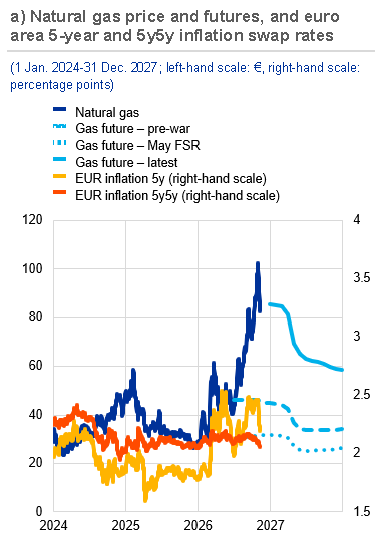
\includegraphics[height=0.60\textheight]{figures/fsr_chart_2_5a.pdf}
\srcline{Source: ECB Financial Stability Review, November 2026, Chart 2.5, panel a (vector crop). Gas: TTF day ahead, \texteuro.}
\end{columns}
\end{frame}

% =====================================================================
\section{Yields}
\begin{frame}{Sovereign yields are near post-crisis highs, and in the euro area inflation and term premia each explain about half of the rise}
\begin{columns}[T,onlytextwidth]
\column{0.55\textwidth}
\footnotesize
\begin{itemize}\setlength{\itemsep}{2pt}
  \item FSR: yields rose together and are close to post-GFC highs, especially at the long end. Markets stayed orderly, but the US Treasury stepped up buybacks of long bonds.
  \item 19 Nov: Bund 10y \BundTenNow\pct{} (17-year high \BundTenPeak\pct{} in late Sep). US Treasuries: 2y \UstTwoNow\pct, 10y \UstTenNow\pct, 30y \UstThirtyNow\pct.
  \item Week to 13 Nov: US 2y $+\UstTwoWeek$\bp, 10y $+\UstTenWeek$\bp. A bear flattening after hot CPI and hawkish Fed comments.
\end{itemize}
\vspace{-4pt}
{\scriptsize
\begin{align*}
y_t^{(n)} &= \underbrace{\tfrac1n\textstyle\sum_{k=0}^{n-1}E_t[r_{t+k}]}_{\text{expectations}}+\underbrace{TP_t^{(n)}}_{\text{term premium}}
&
y_t^{(n)} &\approx \underbrace{r_t^{(n)}}_{\text{real rate}}+\underbrace{\pi_t^{BE,(n)}}_{\text{inflation comp.}}
\end{align*}}
\vspace{-10pt}
\srcline{Right: Fisher relation. FSR real rate: euro area OIS minus inflation-linked swap; US Treasury yield minus break-even. Both split the same yield change: the model split adds up to the fitted change (EA \EaFitted\bp, US \UsFitted\bp), the Fisher split to the observed change (EA \EaObserved\bp, US \UsObserved\bp). Sources: ECB FSR Nov 2026, Section 2.2; Trading Economics and Reuters via Rallies, 19 Nov; US Treasury par yields, 6 to 19 Nov; Reuters via AOL, 16 Nov 2026.}
\column{0.42\textwidth}
\centering
{\scriptsize\textbf{Yield changes since 1 Jan 2026, bp}\par}
\begin{tikzpicture}
\begin{axis}[decomp, ybar stacked, bar width=8pt,
  legend style={font=\tiny, draw=none, fill=none, at={(0.5,-0.12)}, anchor=north, legend columns=2, /tikz/every even column/.append style={column sep=4pt}},
  boxlegend]
  \addplot[fill=accent, draw=none] table[x=x, y=exp]{assets/data/fsr24b.dat};
  \addplot[fill=amber, draw=none] table[x=x, y=tp]{assets/data/fsr24b.dat};
  \addplot[fill=amber!45, draw=none] table[x=x, y=infl]{assets/data/fsr24b.dat};
  \addplot[fill=accent!45, draw=none] table[x=x, y=real]{assets/data/fsr24b.dat};
  \legend{Expectations, Term premium, Inflation comp., Real rate}
  \draw[softgrey!60] (axis cs:-0.7,0) -- (axis cs:7.7,0);
  \draw[softgrey!50, dashed] (axis cs:2,-12) -- (axis cs:2,104);
  \draw[softgrey!50, dashed] (axis cs:5,-12) -- (axis cs:5,104);
  \node[font=\tiny, align=center, text=softgrey] at (axis cs:0.5,98) {10-year\\model split};
  \node[font=\tiny, align=center, text=softgrey] at (axis cs:3.5,98) {10-year\\Fisher split};
  \node[font=\tiny, align=center, text=softgrey] at (axis cs:6.5,98) {30-year\\Fisher split};
\end{axis}
\begin{axis}[decomp, hide axis, /pgf/number format/fixed, /pgf/number format/precision=0]
  \addplot[only marks, mark=diamond*, mark size=2.2pt, black,
    nodes near coords, point meta=y,
    every node near coord/.style={font=\tiny, anchor=south, yshift=1pt}]
    table[x=x, y=total]{assets/data/fsr24b.dat};
\end{axis}
\end{tikzpicture}
\srcline{Diamonds: sum of components. EA to 10 Nov, US to 9 Nov 2026. Rebuilt from the chart data of ECB Financial Stability Review, November 2026, Chart 2.4, panel b. Models: EA \citet{joslin2011}, \citet{geiger2018}; US \citet{adrian2013}, \citet{christensen2012}, \citet{damico2018}.}
\end{columns}
\end{frame}

% =====================================================================
\section{Spreads}
\begin{frame}{France leads the spread widening, and a more fragile investor base raises the risk of abrupt repricing}
\begin{columns}[T,onlytextwidth]
\column{0.55\textwidth}
\footnotesize
\begin{itemize}\setlength{\itemsep}{2pt}
  \item FSR: the OAT-Bund spread rose significantly, with spillovers to other high-debt sovereigns while Bunds gained as a safe haven. Since 2025, spread changes track projected debt-to-GDP, more steeply at the long end.
  \item Market data: OAT-Bund \OatSpreadNow\bp{} on 19 Nov, down from \OatSpreadPeak\bp{} in late Oct, the highest since Nov 2011. BTP-Bund closed at \BtpSpreadSeventeen\bp{} on 17 Nov.
  \item Central banks hold \HoldCbNew\pct{} of euro area sovereign debt (\HoldCbOld\pct{} in 2022), foreign investors \HoldForNew\pct{} (\HoldForOld\pct). With leveraged hedge funds and a quarter of debt due by end-2028, the ECB sees ``the risk of abrupt repricing episodes''.
\end{itemize}
\srcline{BTP: Buoni del Tesoro Poliennali (Italy). OAT: Obligations assimilables du Trésor (France). Bonos: Spanish government bonds. Spread: $s_c=y^{10Y}_c-y^{10Y}_{\text{Bund}}$.\\ Sources: ECB FSR Nov 2026, Section 2.2, Chart 2.6, Box 7; ECB press release and FSR press briefing slide 8 (2022 vs Q2 2026), 18 Nov 2026; Reuters via Rallies, 19 Nov, and via AOL, 16 Nov 2026; SoldiOnline, 17 Nov 2026.}
\column{0.42\textwidth}
\centering
{\scriptsize\textbf{10-year spreads over the Bund, pp}\par}
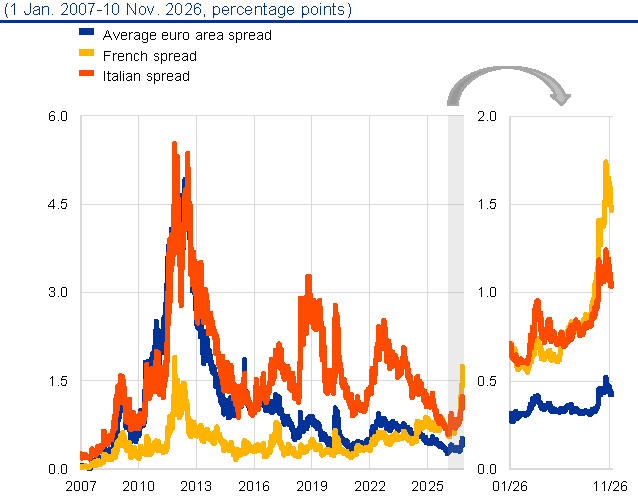
\includegraphics[height=0.40\textheight]{figures/ecb_fsr_briefing_spreads.pdf}
\srcline{1 Jan 2007 to 10 Nov 2026. Source: ECB FSR press briefing, 18 Nov 2026, slide 8 (data of FSR Chart 2.5, panel b), vector crop.}
\vspace{3pt}
{\scriptsize\textbf{Snapshot, 12 Nov 2026 opening, bp}\par}
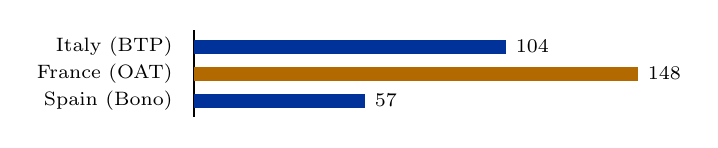
\begin{tikzpicture}
\begin{axis}[xbar, scale only axis, width=0.55\linewidth, height=1.1cm,
  bar width=5pt, bar shift=0pt, xmin=0, xmax=175, ymin=-0.6, ymax=2.6, y dir=reverse,
  ytick={0,1,2}, yticklabels={Italy (BTP), France (OAT), Spain (Bono)},
  tick label style={font=\scriptsize}, xtick=\empty, tick style={draw=none},
  axis x line=none, axis y line*=left, clip=false,
  nodes near coords, every node near coord/.append style={font=\scriptsize}]
  \addplot[fill=accent, draw=none] coordinates {(\SBtp,0)};
  \addplot[fill=amber, draw=none] coordinates {(\SOat,1)};
  \addplot[fill=accent, draw=none] coordinates {(\SBono,2)};
\end{axis}
\end{tikzpicture}
\srcline{Bund \YBund\pct, BTP \YBtp\pct, OAT \YOat\pct, Bono \YBono\pct. Source: QuiFinanza, 12 Nov 2026.}
\end{columns}
\end{frame}

% =====================================================================
\section{Outlook}
\begin{frame}{What to watch in the coming days: data, central bank decisions and the fiscal premium}
\centering
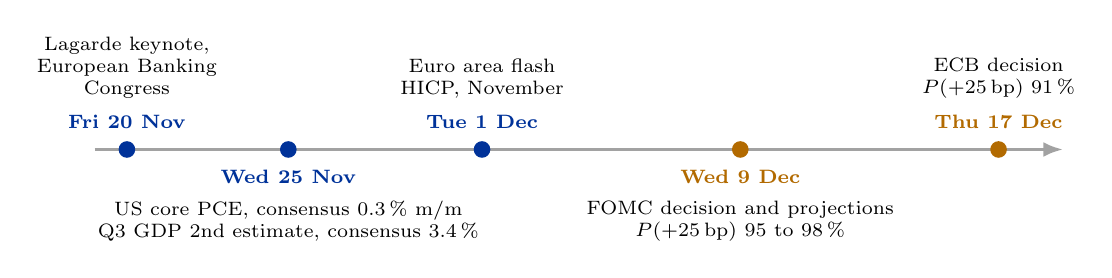
\begin{tikzpicture}[x=4.1mm]
  % x = days after 20 Nov 2026
  \draw[softgrey!60, line width=1.2pt, -{Latex[length=2.5mm]}] (-1,0) -- (29,0);
  \foreach \d/\lab/\txt/\col in {
      0/{Fri 20 Nov}/{Lagarde keynote,\\European Banking\\Congress}/accent,
      11/{Tue 1 Dec}/{Euro area flash\\HICP, November}/accent,
      27/{Thu 17 Dec}/{ECB decision\\$P(+25\,\text{bp})$ \EcbProbHike\pct}/amber} {
    \fill[\col] (\d,0) circle (3pt);
    \node[above=4pt, font=\scriptsize\bfseries, text=\col] (lab) at (\d,0) {\lab};
    \node[above=-1pt, align=center, font=\scriptsize] at (lab.north) {\txt};
  }
  \foreach \d/\lab/\txt/\col in {
      5/{Wed 25 Nov}/{US core PCE, consensus \PceFcst\pct{} m/m\\Q3 GDP 2nd estimate, consensus \GdpFcst\pct}/accent,
      19/{Wed 9 Dec}/{FOMC decision and projections\\$P(+25\,\text{bp})$ \FedProbHikeCme{} to \FedProbHikeLseg\pct}/amber} {
    \fill[\col] (\d,0) circle (3pt);
    \node[below=4pt, font=\scriptsize\bfseries, text=\col] (lab) at (\d,0) {\lab};
    \node[below=-1pt, align=center, font=\scriptsize] at (lab.south) {\txt};
  }
\end{tikzpicture}

\vspace{4pt}
\setbeamerfont{block title}{size=\footnotesize}
\begin{columns}[T,onlytextwidth]
\column{0.32\textwidth}
\begin{block}{Oil and gas prices}
\footnotesize Drive headline HICP and short-term inflation compensation, and with it the size of the December hikes.
\end{block}
\column{0.32\textwidth}
\begin{block}{OAT-Bund spread}
\footnotesize \OatSpreadNow\bp{} on 19 Nov. The French budget and political risk set the fiscal premium.
\end{block}
\column{0.32\textwidth}
\begin{block}{Long-dated auctions}
\footnotesize Demand at the long end shows whether investors still absorb duration without a higher term premium.
\end{block}
\end{columns}

\vspace{2pt}
\quoted{Takeaway: energy keeps policy tight, and fiscal fundamentals decide where the term premium lands.}
\srcline{Sources: ECB weekly schedule (20 Nov) and Governing Council calendar (16 and 17 Dec); Yahoo Finance data calendar, 19 Nov 2026; Eurostat, 18 Nov 2026 (next flash 1 Dec); FOMC meeting calendar; probabilities as on the inflation slide: LSEG via Trading Economics and CME FedWatch via CNBC, 18 Nov 2026.}
\end{frame}

% =====================================================================
\section{References}
\begin{frame}{References (1/2): official sources and data}
\scriptsize\raggedright\setlength{\columnsep}{16pt}
\begin{multicols}{2}
\refitem{ecb2026fsr}
\refitem{ecb2026fsrdata}
\refitem{aguiar2026box7}
\refitem{ecb2026pr}
\refitem{ecb2026briefing}
\refitem{ecb2026mp0910}
\refitem{ecb2026mp1029}
\refitem{ecb2026dfr}
\refitem{ecb2026calendars}
\refitem{eurostat2026flash}
\refitem{eurostat2026final}
\refitem{eurostat2026hicp}
\refitem{fed2026sep}
\refitem{fed2026oct}
\refitem{fed2026cal}
\refitem{ustreasury2026}
\end{multicols}
\end{frame}

\begin{frame}{References (2/2): market news and term-structure models}
\scriptsize\raggedright\setlength{\columnsep}{16pt}
\begin{multicols}{2}
\refitem{reuters2026aol}
\refitem{reuters2026rallies}
\refitem{te2026bund}
\refitem{cnbc2026}
\refitem{stockanalysis2026cpi}
\refitem{quifinanza2026}
\refitem{soldionline2026}
\refitem{yahoo2026}
\refitem{adrian2013}
\refitem{christensen2012}
\refitem{damico2018}
\refitem{geiger2018}
\refitem{joslin2011}
\end{multicols}
\end{frame}

\end{document}
